During development of this project, we faced many difficulties in implementing the initial scope of our project. The primary and insurmountable hurdle we faced was with data. In our initial proposal, we believed that we could make the recommender model multilingual, and able to understand queries from multiple languages. We primarily focussed on English, Sinhala, and Tamil as our languages of choice, as they are the main three languages of Sri Lanka.

We utilized various datasets to train our models. From datasets pre-made for the purposes of training AI, to data database dumps of popular online libraries, we had no problems finding ready-to-use data for training our recommender in English. The problems arose when we tried to create datasets in Sinhala and Tamil languages.

Towards this end, we requested the assistance of the National Library of Sri Lanka, and obtained their Sri Lanka National Bibliography (Data from January 2000, to June 2022). This is a compedium of 22 years of every book published in Sri Lanka, and the data was available trilingually. The majority of the data is in digitally typed PDFs, while some of the older SLNB volumes are Scanned PDFs of the original print volumes. Even with the digital PDFs, the bibliography entries are incredibly hard to parse.

\begin{figure}[htbp]
    \centering
    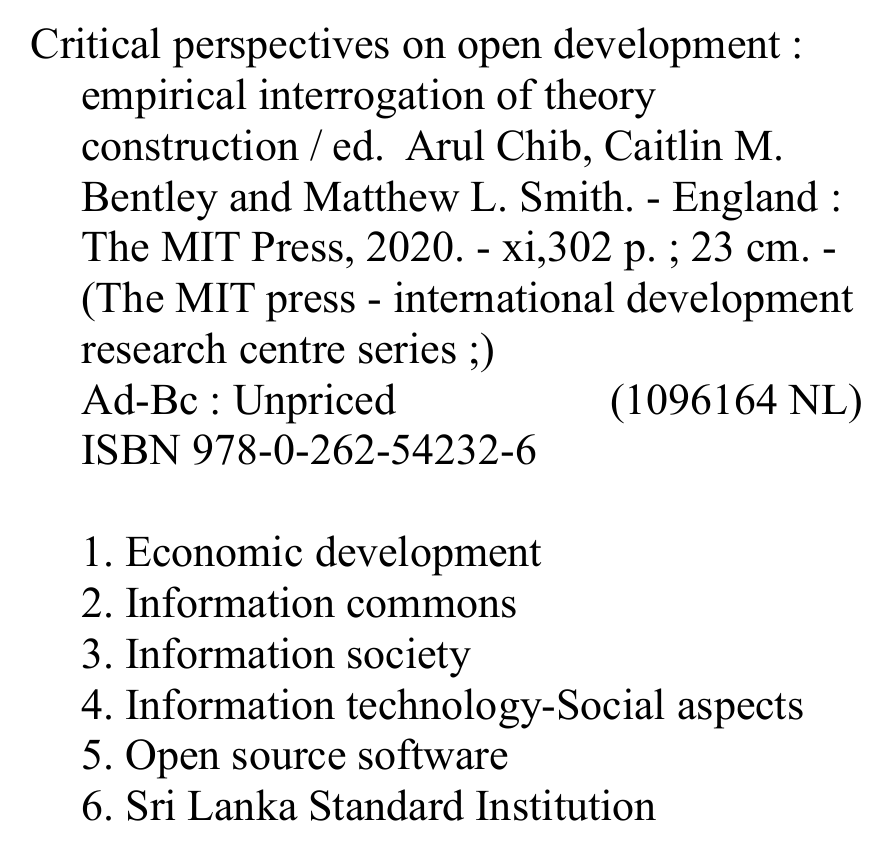
\includegraphics[width=0.5\textwidth]{../../assets/snlb_entry.png}
    \caption{A page of bibliographies}
    \label{fig:slnbpage}
\end{figure}

As you can see from the above bibliography page, the bibliographies are given in a two column layout, with the bibliographies themselves having no consistent format.

\begin{figure}[htbp]
    \centering
    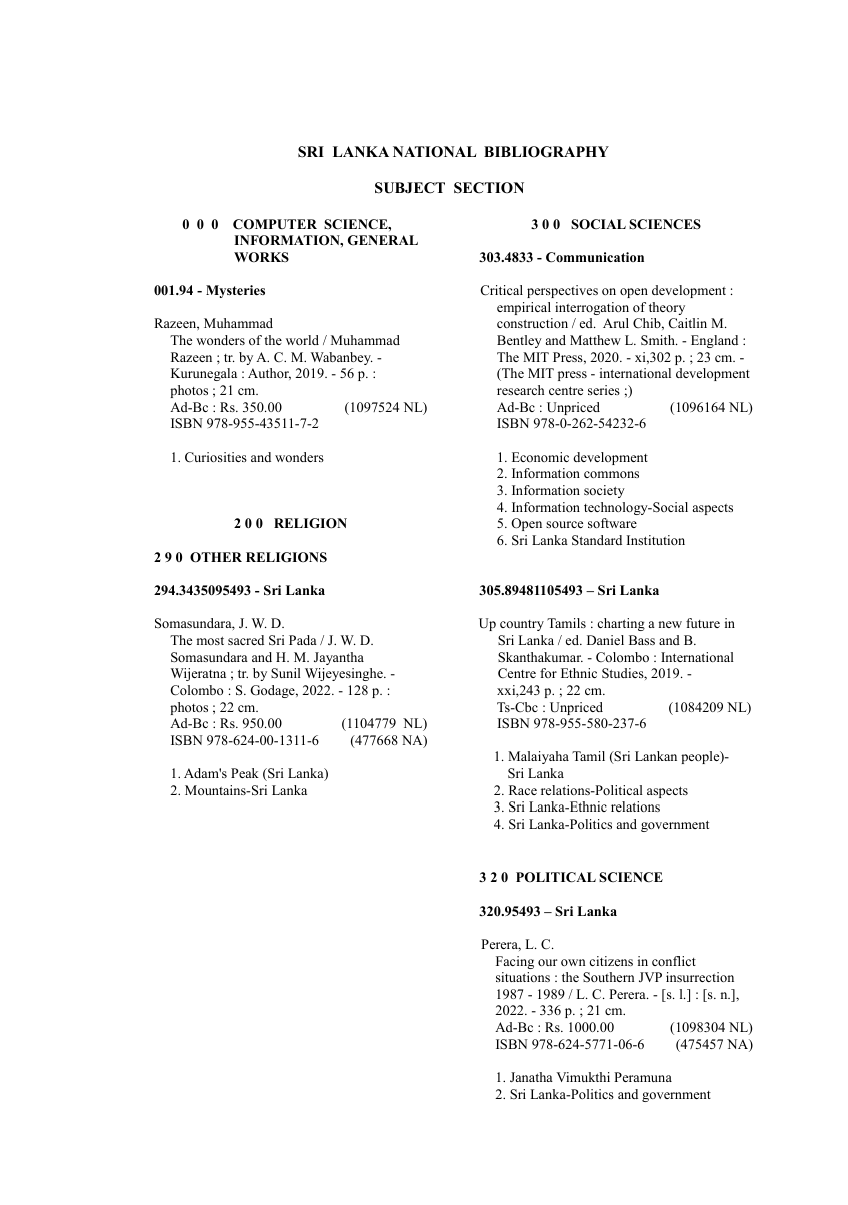
\includegraphics[width=1\textwidth]{../../assets/slnb_june_pg47.png}
    \caption{A page of bibliographies}
    \label{fig:slnbpage}
\end{figure}

The problem is made worse by the fact that, with the way the PDF is made, the two column layout is not parsed properly by pdf analysis algorithms. This makes it such that data from two colums are mashed up together, creating an unreadable jumble of text. In order to utilize this resource, a massive undertaking to extract, clean, and standardize the text would have to be attempted.

Upon research, we believe that mass scale datasets used by companies such as OpenAI, Google, Amazon, and Microsoft are mostly created by hand. A novel technique for utilizing an AI preprocessor model to create structured data from internet scale mass data was proposed by OpenAI, and we feel that the approach used there (manually generate 20\% of the data, have the preprocessor model extract the rest) would have been effective, but hardware constraints limited us in the exploration of this technique.
The technique proposed by OpenAI leverages a structured dataset which is used to train a model to extract data from internet-scale data. This data is obtained by mass scale human workers, obtained through the Amazon M-Turk program. All in all, the paper estimates that they spent roughly 10,000 US Dollars to extract 70,000 points of data. That computes to around Rs.3,000,000, or 3 Million Rupees.

A large scale orchestrated effort to parse this data into a machine readable format would prove useful for further research into LLMs and Deep Neural networks which can parse and understand Sinhala and Tamil languages, but is beyond the scope of this project at this time.

While our initial goal was to extract this data and store it in a immutable datastore like Blockchain or IPFS, we were ultimately unable to do so due to the aforementioned issues with data extraction. We hope that our work so far will prove useful to researchers and developers in the future hoping to work on this same matter.

Further, we faced a plethora of issues when it comes to collaboration. Due to our relative inexperience with Git, managing the various branches, tracking, and updating them, and merging changes was handled haphazardly. The availability of \texttt{git cherry-pick} was sadly realized a very late stage in the project, and this caused a few members contributions to not be recorded in Github's statistics, as some code was overwritten and files moved around in the final rush to organize and present the code.

\subsubsection*{Further Progress}
We do believe that our work has many avenues for improvement and further development. With better hardware, we believe that the BERT based ML Recommender model can be deployed successfully, and the DistilBert model could be used in a production environment without too much hassle.

Further, we believe that utilizing manpower to parse and analyze the SLNB data would prove a very fruitful endeavour. The data can be used for applications well beyond what is in this scope of this Software Development project, and will serve our mother country well.

It is also our aim to package the api server into a ready-to-go Docker Image. A docker image is already provided with the project files, but we feel that the API server could be improved further with more modular design, and with the option of adding many more models, and even using a bring-your-own-model sort of system. As long as the recommendation, user data, and metadata formats remain consistent, all deployments can talk to each other and exchange data to boost productivity.